%!LW recipe=pdflatex → makeglossaries → biber → pdflatex ×2
\documentclass[12pt]{article}

% Essential Packages
\usepackage{xcolor}
\usepackage[main=slovak,english]{babel}
\usepackage{setspace}
\usepackage{newtxtext}
\usepackage[a4paper, left=3.5cm, right=2cm, top=2.5cm, bottom=2.5cm]{geometry}
\usepackage{graphicx}
\usepackage{pdfpages}
\usepackage{tocbibind}
\usepackage{fancyhdr}
\usepackage{longtable}
\usepackage[acronym]{glossaries}
\usepackage{url}
\usepackage{caption}
\usepackage[T1]{fontenc}
\usepackage[utf8]{inputenc}
\usepackage{csquotes}
\usepackage{array}
\usepackage{listings}
\usepackage{comment}
\usepackage{algorithm}
\usepackage{algpseudocode}

% Thesis type
\def\isBachelorThesis{1}

% Thesis metadata
\ifdefined\isBachelorThesis
\title{Spracovanie údajov pre modelovanie narušenia informácie uchovávanej v pamäti DNA typu nanopór}
\author{Patrik Homola}
\def\thesisHeader{Bakalárska práca}
\fi

\def\uid{FI-11145-18967}
\def\supervisor{doc. RNDr. Peter Farkas, PhD.}
\def\consultant{Mgr. Peter Jarnvars}
\def\thesisyear{2026}

\def\university{PANEURÓPSKA VYSOKÁ ŠKOLA}
\def\faculty{Fakulta Informatiky}
\def\program{Aplikovaná informatika}
\def\fieldofstudy{Informatika}
\def\department{Ústav aplikovanej informatiky}

\usepackage[
    backend=biber,
    style=iso-numeric,
]{biblatex}
\addbibresource{essentials/bibliography.bib}

\onehalfspacing
\pagestyle{fancy}
\fancyhead{}
\fancyfoot{}
\fancyfoot[R]{\thepage}
\renewcommand{\headrulewidth}{0pt}

\makeglossaries
\loadglsentries{essentials/acronyms}

\captionsetup{
    justification=raggedright,
    singlelinecheck=false
}

\setkeys{Gin}{width=0.9\textwidth}
\makeatletter
\g@addto@macro\@floatboxreset{\centering}
\makeatother

\lstset{
    basicstyle=\ttfamily\small,
    breaklines=true,
    showstringspaces=false,
    keywordstyle=\color{blue},
    commentstyle=\color{green!60!black},
    stringstyle=\color{red},
    backgroundcolor=\color{gray!10},
    frame=single,
    framesep=5pt
}

\renewcommand{\lstlistingname}{Výpis}
\renewcommand{\lstlistlistingname}{Zoznam výpisov}

\begin{document}
\selectlanguage{slovak}

% Essentials
\include{essentials/titlepage}
\include{essentials/titlepage-alt}
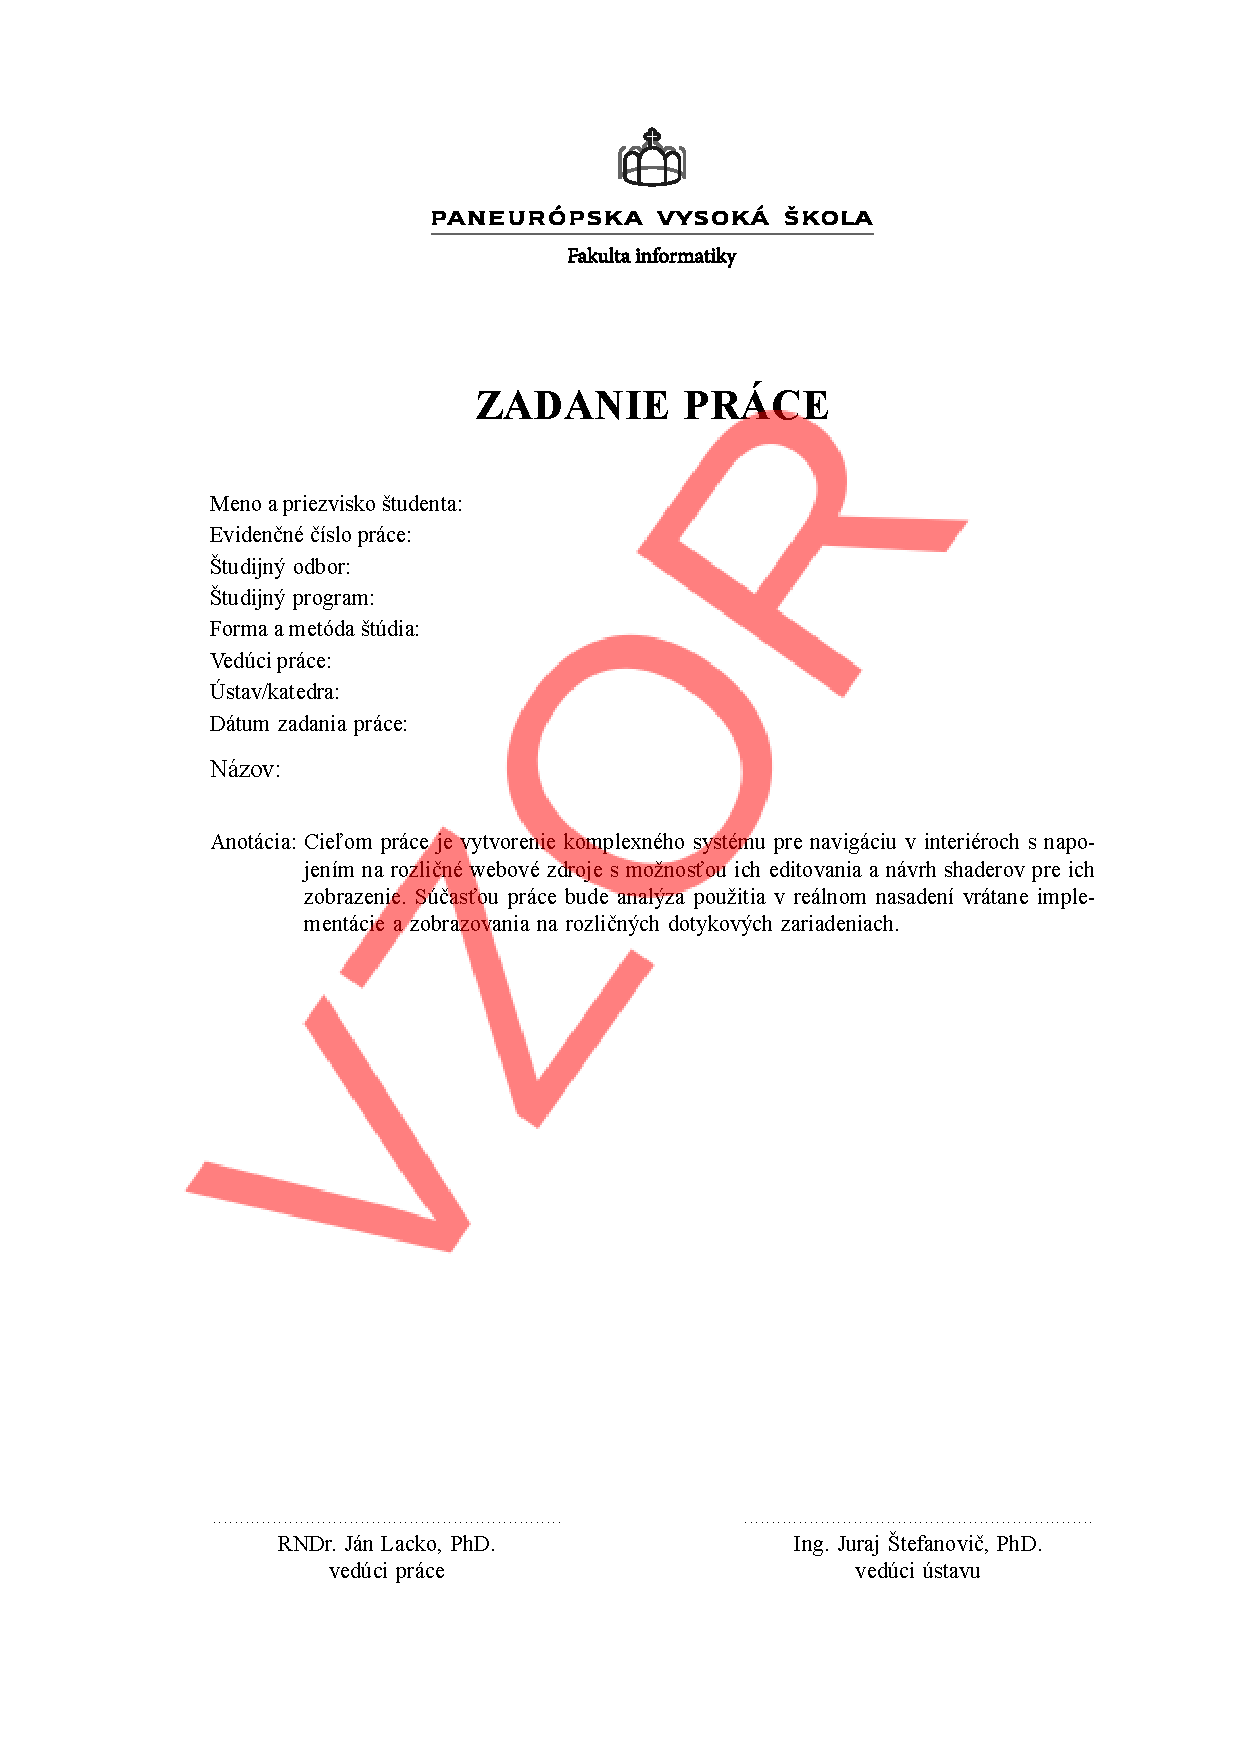
\includepdf{essentials/assignment.pdf}
\begin{flushleft}
    \vspace*{\fill}
    \textbf{Poďakovanie:}\\
    \vspace{1em}
Pri vypracovaní tejto práce by som sa rád poďakoval za odbornú pomoc pánom \supervisor a \consultant, ktorí mi poskytli mnoho cenných rád a konzultácií.
\vspace{1em}\\
\end{flushleft}


\include{essentials/declaration}
% Redefine the abstract environment to align the title and content to the left
\makeatletter
\renewenvironment{abstract}{
    \if@twocolumn
        \section*{\abstractname}%
    \else
        \normalfont\small
        \begin{flushleft} % Change from center to flushleft
            {\bfseries \abstractname\par}%
        \end{flushleft}%
        \noindent\raggedright
    \fi
}
{
    \if@twocolumn\else\par\fi
}
\makeatother

\begin{abstract}

Táto bakalárska práca sa zaoberá spracovaním sekvenačných dát z nanopórového sekvenovania s cieľom 
vytvoriť nástroje a metódy na získanie DNA reťazcov vhodných pre modelovanie narušenia informácie 
v DNA kanáloch. Práca opisuje navrhnutý a implementovaný pipeline, ktorý transformuje surové elektrické 
signály vo formáte pod5 na zarovnané a zklasifikované DNA sekvencie. Kľúčovými komponentmi riešenia 
sú konverzia dát z formátu BAM do textovej podoby, viacnásobné zarovnanie sekvencií pomocou vlastného 
algoritmu inšpirovaného beam search prístupom a identifikácia primeru bez predchádzajúcej znalosti 
jeho presnej sekvencii. Práca demonštruje, že zo surového signálu je možné získať relevantné DNA 
reťazce, ktoré tvoria spoľahlivý základ pre charakterizáciu chybovosti nanopórového čítania. Navrhnutý 
metodický a implementačný rámec umožňuje pokračovať v ďalšom výskume smerom k presnejšiemu modelovaniu 
narušenia informácie v DNA pamätiach.

\smallskip

\noindent\textbf{Kľúčové slová:} nanopórové sekvenovanie, spracovanie DNA dát, zarovnanie sekvencií, DNA pamäť, modelovanie chýb

\end{abstract}
\pagebreak
\begin{otherlanguage}{english}
\begin{abstract}

This bachelor thesis addresses the processing of sequencing data from nanopore sequencing with the goal 
of creating tools and methods to obtain DNA sequences suitable for modeling information perturbation in DNA 
channels. The thesis describes a proposed and implemented pipeline that transforms raw electrical signals 
in pod5 format into aligned and classified DNA sequences. Key components of the solution are conversion of 
data from BAM format to text representation, multiple sequence alignment using a custom algorithm inspired 
by the beam search approach, and primer identification without prior knowledge of its exact sequence. The 
work demonstrates that from raw signal it is possible to obtain relevant DNA sequences that form a reliable 
basis for characterizing the error rate of nanopore reading. The proposed methodological and implementation 
framework enables further research towards more accurate modeling of information perturbation in DNA storage 
systems.

\smallskip

\noindent\textbf{Keywords:} nanopore sequencing, DNA data processing, sequence alignment, DNA storage, error modeling

\end{abstract}
\end{otherlanguage}

\tableofcontents
\pagebreak
\listoffigures
\pagebreak
\lstlistoflistings
\pagebreak

\glsaddall
\addcontentsline{toc}{section}{Zoznam skratiek a značiek}
\printglossary[type=\acronymtype,title={Zoznam skratiek a značiek}]

%%%%%%% DOCUMENT BODY %%%%%%%

\section{Úvod}
V dnešnej digitálnej dobe sa množstvo generovaných dát exponenciálne zvyšuje,
čo vytvára potrebu efektívnych a trvalo udržateľných metód ich ukladania.
Tradičné úložné médiá, ako sú pevné disky, SSD disky a magnetické pásky,
majú obmedzenú životnosť a kapacitu, čo vedie k častým migráciám dát
a zvýšeným nákladom na údržbu.

DNA ako médium pre ukladanie dát ponúka niekoľko významných výhod:
\begin{itemize}
    \item \textbf{Vysoká hustota ukladania:} Hustota informácií v DNA je extrémne vysoká. Len 5 gramov DNA obsahuje približne $4\cdot10^{21}$ nukleotidov, čo by teoreticky mohlo uchovať $8\cdot10^{21}$ bitov, alebo jeden zettabyte \cite{Arxiv221105552DNAStorage}.
    To znamená, že obrovské množstvo informácií môže byť uložené v mimoriadne malom objeme.
    \item \textbf{Dlhodobá stabilita:} DNA je chemicky stabilná molekula, ktorá môže prežiť tisíce rokov za správnych podmienok. Na rozdiel od tradičných médií, ktoré sa môžu degradovať počas niekoľkých dekád, DNA môže uchovávať dáta po veľmi dlhú dobu bez straty integrity.
    \item \textbf{Energetická efektívnosť:} Ukladanie dát do DNA nevyžaduje neustálu energiu na udržiavanie dát, na rozdiel od elektronických úložísk, ktoré potrebujú napájanie na zachovanie informácií. To vedie k výrazným úsporám energie a znižuje ekologickú stopu dátových centier.
    \item \textbf{Ľahká replikácia a prenosnosť:} DNA môže byť ľahko kopírovaná pomocou biologických procesov, čo umožňuje jednoduché zálohovanie a prenos dát medzi rôznymi miestami bez potreby špecializovaného hardvéru.
    \item \textbf{Odolnosť voči technologickému zastaraniu:} Na rozdiel od tradičných úložných médií, ktoré môžu rýchlo zastarať v dôsledku technologického pokroku, DNA ako médium zostáva nezmenené a čitateľné pomocou základných biologických techník.
\end{itemize}

Napriek uvedeným výhodám proces čítania DNA pomocou nanopórov prináša špecifické výzvy.
Pri sekvenovaní DNA cez nanopór sa DNA molekula prechádza cez nanopór po jednotlivých nukleotidoch,
pričom elektrický signál identifikuje bázy.
%todo: doplniť odkaz na sekciu o nanopórovom sekvenovaní
Podrobnejšie vysvetlenie tejto technológie bude uvedené v sekcii \ref{sec:nanopore_sequencing}.     
 Tento proces je však náchylný na chyby,
keďže DNA sa môže pohybovať rýchlo alebo nepravidelne, čo vedie k nesprávnemu
určeniu sekvencie nukleotidov. Tieto chyby v čítaní majú priamy vplyv na integritu
uložených dát a vyžadujú sofistikované metódy kódovania a korekcie chýb.
S pokračujúcim vývojom technológií nanopórového sekvenovania sa
presnosť postupne zvyšuje, čo robí z DNA perspektívnu alternatívu k tradičným metódam ukladania dát.

Cieľom tejto práce je prispieť k zefektívneniu procesu ukladania
dát do DNA vytvorením modela narušenia, ktorý popisuje chyby vznikajúce pri čítaní a zápise dát.
Pochopením a formalizáciou týchto narušení je možné zvýšiť spoľahlivosť a presnosť ukladania
a načítavania informácií, čo je kľúčové pre praktické využitie DNA ako úložného média v budúcnosti.

Model narušenia opisuje pravdepodobnostné správanie chýb, ktoré vznikajú počas syntézy,
sekvenovania a uchovávania DNA molekúl. Tento model zachytáva typy chýb ako substitúcie,
inzercie a delécie nukleotidov, čím poskytuje základ pre návrh efektívnych kódovacích
a opravných schém pri ukladaní dát do DNA.



\section{Teoretické východiská}
\subsection{Biologické východiská}
Biologická syntéza DNA je proces,
pri ktorom DNA polymeráza vytvára
nový reťazec na základe templátového vlákna, pričom syntéza
prebieha výlučne v smere 5'$\rightarrow$3'. Kľúčovou podmienkou začatia
syntézy je prítomnosť primeru, teda krátkeho komplementárneho
oligonukleotidu, ktorý sa naviaže na templát a poskytne voľnú
3'-OH skupinu potrebnú pre katalytickú aktivitu polymerázy.
Po naviazaní primeru polymeráza postupne inkorporuje deoxyribonukleotidy
podľa pravidiel komplementárneho párovania báz (A--T, G--C), čím predlžuje
vznikajúci reťazec DNA. Tento proces je nevyhnutný pre replikáciu DNA, ktorá je základom
prenosu genetickej informácie.

\subsubsection{Smer reťazca: 5'$\rightarrow$3' a 3'$\rightarrow$5'}
DNA reťazec má chemickú polaritu --- jeden koniec reťazca má voľnú fosfátovú skupinu na 5' uhlíku cukru (5' koniec) a druhý koniec má voľnú hydroxylovú skupinu na 3' uhlíku (3' koniec).

\begin{itemize}
    \item \textbf{Smer 5'$\rightarrow$3'} --- smer, v ktorom DNA polymeráza syntetizuje nový reťazec. Polymeráza číta templát v smere 3'$\rightarrow$5' a zapisuje nový reťazec v smere 5'$\rightarrow$3'.
    \item \textbf{Smer 3'$\rightarrow$5'} --- smer čítania templátového vlákna počas syntézy. Nie je možné syntetizovať reťazec v tomto smere priamo.
\end{itemize}

Táto polarita má priamy dopad na nanopórové sekvenovanie --- tá istá DNA molekula môže vstúpiť do nanopóru z ľubovoľného konca, čím vznikajú čítania v oboch smeroch (forward aj reverse). Pri spracovaní dát je preto potrebné uvažovať s oboma orientáciami.

\subsubsection{Simplexný a duplexný reťazec}
\begin{itemize}
    \item \textbf{Simplex (ssDNA)} --- jednoreťazcová DNA. Obsahuje iba jedno vlákno nukleotidov. Vyskytuje sa napríklad počas replikácie alebo pri niektorých vírusoch. V kontexte nanopórového sekvenovania sa čítanie vykonáva práve na jednoreťazcovej forme.
    \item \textbf{Duplex (dsDNA)} --- dvojreťazcová DNA. Dve komplementárne vlákna sú navzájom spojené vodíkovými väzbami medzi pármi báz (A--T, G--C) a tvoria charakteristickú dvojitú špirálu (double helix). Toto je štandardná forma, v ktorej je DNA uložená v bunke.
\end{itemize}

Pri biosyntéze DNA vzniká z jednoreťazcového templátu nový komplementárny reťazec --- výsledkom je duplexná DNA. Pre každý pôvodný reťazec tak existuje komplementárny reťazec s opačnou polaritou. To znamená, že pri nanopórovom sekvenovaní môžeme naraziť na štyri varianty toho istého úseku DNA:
\begin{enumerate}
    \item pôvodný reťazec v smere 5'$\rightarrow$3',
    \item pôvodný reťazec v smere 3'$\rightarrow$5' (reverzný),
    \item komplementárny reťazec v smere 5'$\rightarrow$3',
    \item komplementárny reťazec v smere 3'$\rightarrow$5' (reverzný komplement).
\end{enumerate}

Tieto štyri varianty sú kľúčovým zdrojom komplikácií pri klastrovacích algoritmoch --- sekvencie reprezentujúce rovnaký úsek DNA môžu byť sekvenerom prečítané v rôznych formách a bez primerov ich nie je možné jednoducho stotožniť.


\subsection{Nanopórové sekvenovanie}
Nanopore sekvenovanie je technológia používaná na sekvenovanie DNA a RNA molekúl \cite{Zheng2023Nanopore}. Táto metóda umožňuje čítanie genetického materiálu tým, že molekuly prechádzajú cez nanometrové póry (nanopóry), čo vedie k zmene elektrického prúdu, ktorý je následne analyzovaný na určenie sekvencie nukleotidov \cite{Zheng2023Nanopore}.
Je to revolučná technológia v oblasti genomiky, ktorá umožňuje rýchle a presné sekvenovanie s minimálnymi nákladmi a zariadeniami prenosných veľkostí \cite{Zheng2023Nanopore}.
Aplikácie nanopórového sekvenovania zahŕňajú diagnostiku chorôb, výskum genetických porúch a monitorovanie environmentálnych vzoriek \cite{Zheng2023Nanopore}.

Nanopórové sekvenovanie je obzvlášť užitočné pre jeho schopnosť čítať dlhé sekvencie DNA, čo zjednodušuje zostavovanie genómov a identifikáciu štruktúrnych variácií \cite{Zheng2023Nanopore,Lopez2019DNA}.
Funguje na princípe detekcie zmien v elektrickom prúde, keď molekula prechádza cez nanopór, čo umožňuje priame čítanie sekvencií bez potreby amplifikácie alebo značenia \cite{Zheng2023Nanopore}.
DNA alebo RNA molekuly sú vedené cez nanopór pomocou elektrického poľa, pričom každá báza spôsobuje charakteristickú zmenu prúdu, ktorá je zaznamenaná a analyzovaná softvérom na určenie sekvencie \cite{Zheng2023Nanopore}.

\subsection{Prekladanie DNA/mRNA do signálu}
Prekladanie DNA alebo RNA sekvencií do elektrického signálu v nanopórovom sekvenovaní \cite{Zheng2023Nanopore} zahŕňa niekoľko kľúčových krokov:
\begin{itemize}
    \item \textbf{Príprava vzorky:} DNA alebo RNA molekuly sú pripravené na sekvenovanie, často zahŕňajúce fragmentáciu a pridanie adaptérnych sekvencií.
    \item \textbf{Vedenie cez nanopór:} Molekuly sú vedené cez nanopór pomocou elektrického poľa, ktoré spôsobuje ich pohyb \cite{Zheng2023Nanopore}.
    \item \textbf{Detekcia prúdu:} Keď molekula prechádza cez nanopór, každá báza spôsobuje charakteristickú zmenu v elektrickom prúde, ktorý je zaznamenaný ako časová séria dát \cite{Zheng2023Nanopore}.
    \item \textbf{Analýza signálu:} Zaznamenaný elektrický signál je analyzovaný pomocou algoritmov na identifikáciu sekvencie nukleotidov na základe zmien prúdu \cite{Zheng2023Nanopore}.
    \item \textbf{Preklad do sekvencie:} Softvér prekladá analyzovaný signál späť do sekvencie DNA alebo RNA, čo umožňuje výskumníkom získať genetické informácie z pôvodnej molekuly \cite{Zheng2023Nanopore}.
\end{itemize}

Výstupom z procesu nanopórového sekvenovania je sekvencia nukleotidov (A, T, C, G pre DNA alebo A, U, C, G pre RNA) reprezentujúca genetickú informáciu pôvodnej molekuly \cite{Zheng2023Nanopore}.
Tento výstup je často vo forme textového súboru (napríklad FASTQ formát), ktorý obsahuje sekvencie spolu s kvalitatívnymi skóre pre každú bázu \cite{Zheng2023Nanopore}.
Vzhľadom na technické obmedzenia a variabilitu v procese sekvenovania je bežné, že jednotlivé DNA alebo RNA reťazce sú prečítané niekoľkokrát (tzv. \enquote{coverage} alebo \enquote{depth of coverage}) \cite{Zheng2023Nanopore}.
Toto opakované čítanie zvyšuje spoľahlivosť a presnosť výslednej sekvencie, pretože umožňuje korekciu chýb a identifikáciu variácií v genetickom materiáli \cite{Zheng2023Nanopore,Lopez2019DNA}.
Napriek tomu, že sa reťazce čítajú viackrát, stále môže dôjsť k nepresnostiam v sekvencii v dôsledku šumu v signáli \cite{Zheng2023Nanopore}.

Reťazce DNA alebo RNA môžu byť čítané rôznou rýchlosťou počas nanopórového sekvenovania, čo môže ovplyvniť kvalitu a presnosť zaznamenaného signálu \cite{Zheng2023Nanopore}.
Rýchlosť prechodu molekuly cez nanopór je ovplyvnená viacerými faktormi, vrátane veľkosti molekuly, jej konformácie, interakcií s nanopórom a podmienok prostredia (napríklad teplota a iónová sila) \cite{Zheng2023Nanopore}.

Keďže DNA a RNA molekuly sú veľmi malé, signál zaznamenaný počas nanopórového sekvenovania odráža interakcie jednotlivých nukleotidov (báz) s nanopórom \cite{Zheng2023Nanopore}.
Každá báza má jedinečný tvar a elektrické vlastnosti, ktoré ovplyvňujú spôsob, akým mení elektrický prúd pri prechode cez nanopór \cite{Zheng2023Nanopore}.
Preto je možné získať signál pre každú jednotlivú bázu v molekule, čo umožňuje presné čítanie sekvencie \cite{Zheng2023Nanopore}.


\subsection{Basecalling nástrojom Dorado}
\input{chapters/04_PraktickaRealizacia/Dorado_atoms/01_co_je_dorado}

\subsection{Klastrovanie sekvencií}
Klastrovací algoritmus je metóda, ktorá rozdeľuje množinu dát do skupín (klastrov) tak, aby dáta v rámci jednej skupiny boli si navzájom podobné a dáta z rôznych skupín boli odlišné \cite{Qu2022Clover}. Tieto algoritmy sa často používajú v bioinformatike na analýzu sekvencií DNA alebo iných biologických dát.

Clover algoritmus je efektívny klastrovač navrhnutý špeciálne pre DNA sekvencie v oblasti DNA-based data storage. Využíva stromovú štruktúru na rýchle a presné zoskupovanie sekvencií podľa ich podobnosti, čím zvyšuje efektivitu a škálovateľnosť procesu \cite{Qu2022Clover}. Clover umožňuje efektívne spracovanie veľkých množín sekvencií a je vhodný pre moderné aplikácie v oblasti ukladania dát do DNA.

Clover algoritmus Klastruje sekvencie DNA na zaklade ako zacinaju a to tak ze ich usporiada do stromovej struktury podobnemu trie.

clover berie data vo forme kde kazdy riadok bude obsahovat id a dna sekvenciu.


\subsection{Viacnásobné zarovnanie sekvencií}
Viacnásobné zarovnanie sekvencií (Multiple Sequence Alignment, MSA) je proces usporiadania troch alebo viacerých biologických sekvencií (DNA, RNA alebo proteínov) tak, aby boli identifikované podobné regióny medzi nimi. Tieto podobnosti môžu odhaliť štrukturálne, funkčné alebo evolučné vzťahy medzi sekvenciami.

\subsubsection{Základný princíp}
Pri viacnásobnom zarovnaní sekvencií hľadáme také usporiadanie, ktoré maximalizuje podobnosť medzi všetkými sekvenciami súčasne. Do sekvencií sú vkladané medzery (gap characters, značené pomlčkou `-`), aby sa zodpovedajúce pozície dostali do rovnakých stĺpcov.

\paragraph{subsubsubsection}{Príklad zarovnania}
Majme tri jednoduché sekvencie:
\begin{itemize}
    \item Sekvencia 1: \texttt{ACGT}
    \item Sekvencia 2: \texttt{AGT}
    \item Sekvencia 3: \texttt{ACCT}
\end{itemize}

Ich zarovnanie môže vyzerať nasledovne:

\begin{verbatim}
Seq1: A C G T
Seq2: A - G T
Seq3: A C C T
\end{verbatim}

\subsubsection{Význam a využitie}
Viacnásobné zarovnanie má niekoľko dôležitých aplikácií:

\begin{itemize}
    \item \textbf{Fylogenéza} -- konštrukcia evolučných stromov
    \item \textbf{Identifikácia konzervovaných motívov} -- nálezenie funkčne dôležitých oblastí
    \item \textbf{Predikcia štruktúry} -- odvodenie sekundárnej a terciárnej štruktúry proteínov
    \item \textbf{Homológia} -- určenie príbuznosti medzi sekvenciami
\end{itemize}

\subsubsection{Zložitosť problému}
Viacnásobné zarovnanie je výpočtovo náročný problém. Presné riešenie pomocou dynamického programovania má časovú zložitosť $O(L^n)$, kde $L$ je dĺžka sekvencií a $n$ je ich počet. Preto sa v praxi používajú heuristické algoritmy.

\subsubsection{Skórovacia funkcia}
Kvalita zarovnania sa hodnotí pomocou skórovacej funkcie, ktorá typicky obsahuje:

\begin{itemize}
    \item \textbf{Match score} -- bodovanie zhody medzi znakmi
    \item \textbf{Mismatch penalty} -- penalizácia za nezhodu
    \item \textbf{Gap penalty} -- penalizácia za medzery (môže byť lineárna alebo afinná)
\end{itemize}

\subsubsection{Bežné algoritmy}
Medzi najpoužívanejšie algoritmy pre MSA patria:

\begin{itemize}
    \item \textbf{ClustalW/ClustalOmega} -- progresívne zarovnanie pomocou sprievodného stromu
    \item \textbf{MUSCLE} -- rýchly progresívny algoritmus s iteratívnym spresňovaním
    \item \textbf{T-Coffee} -- kombinuje párové zarovnania do finálneho MSA
    \item \textbf{MAFFT} -- využíva FFT pre rýchle nálezenie homológnych oblastí
\end{itemize}



\section{Ciele práce a vstupné dáta}
\subsection{Ciele práce}
Cieľom tejto úlohy je simulovať chyby, ktoré vznikajú pri čítaní DNA pomocou nanopórového sekvenovania.
Nanopórové sekvenovanie je inovatívna technológia, ktorá umožňuje rýchle a efektívne čítanie genetického materiálu.

Úlohou je vytvoriť generátor, ktorý na základe pravdepodobnosti chyby náhodne pridáva chyby do reálneho DNA reťazca. Tento generátor by mal byť schopný simulovať rôzne typy chýb, ako sú záměny báz, vloženia alebo vynechania báz, ktoré sa môžu vyskytnúť počas procesu sekvenovania.

Táto simulácia bude slúžiť na testovanie a vyhodnocovanie algoritmov pre spracovanie sekvenačných dát, ktoré musia byť robustné voči týmto chybám. Cieľom je zlepšiť presnosť a spoľahlivosť analýzy genetických informácií získaných pomocou nanopórového sekvenovania.


\subsection{Vstup a požadovaný výstup}
TODO: NADVIAZ
\subsubsection{Vstup}
Cieľ výstupu analýzy DNA získaných pomocou nanopórového sekvenovania je určiť vzťah medzi pôvodným DNA reťazcom a jeho pozorovanými čítaniami, ktoré vznikajú počas sekvenovania.
Namiesto priameho priraďovania konkrétneho referenčného reťazca k jednotlivým čítaniam je zvolený opačný postup: 
z dostupných nanopórových čítaní sa odhaduje najpravdepodobnejšia pôvodná sekvencia.
Tento odhad je založený na identifikácii dostatočne veľkej množiny podobných sekvencií, pri ktorých možno predpokladať spoločný pôvod.
Následne sa pre takúto skupinu vypočíta konsenzus, ktorý by mal byť čo najbližšie pôvodnému DNA reťazcu.

\textit{Konsenzus} je syntetizovaná sekvencia zložená z nukleotidov, ktoré sa v každej pozícii zarovnaných sekvencií vyskytujú s najväčšou frekvenciou.
Inými slovami, pre každú pozíciu v zarovnaní sa vyberie báza (A, C, G alebo T), ktorá sa v danej pozícii objavuje najčastejšie vo všetkých zarovnaných čítaniach.
Konsenzus tak reprezentuje najlepší odhad pôvodnej DNA sekvencie na základe dostupných pozorovaní a ich spoľahlivosti.

Keďže DNA reťazce sú dlhé a jednotlivé čítania obsahujú chyby, sekvencie sa môžu navzájom líšiť a byť vzájomne posunuté.
Z tohto dôvodu je potrebné vykonať viacnásobné zarovnanie sekvencií (multiple sequence alignment), aby sa konsenzus určoval z nukleotidov nachádzajúcich sa v rovnakých pozíciách.

Takto definovaný výstup umožňuje vytvoriť pravdepodobnostný model čítania DNA k-tíc (k-merov).
Tento model sa interpretuje ako komunikačný kanál a vychádza z matematickej teórie komunikácie \\cite{Shannon1948Communication}.
Namiesto jedného pevného výsledku sa každej k-tici priraďuje rozdelenie možných prečítaných sekvencií.
Formálne môžeme písať
$$
X=\Sigma^k,\quad Y=\Sigma^*,\quad K(y\mid x)=\Pr(Y=y\mid X=x),
$$
kde $\Sigma=\{A,C,G,T\}$, $x\in\Sigma^k$ je pôvodná k-tica a $y\in\Sigma^*$ je prečítaná sekvencia.
Tá môže mať aj inú dĺžku v dôsledku delécií alebo inzercií.

Pre konkrétnu k-ticu, napríklad $x=\mathrm{ATCG}$, môže byť rozdelenie nasledovné:
$$
\Pr(Y=\mathrm{ATCG}\mid X=x)=0.33,
$$
$$
\Pr(Y=\mathrm{ATTCG}\mid X=x)=0.20,
$$
$$
\Pr(Y=\mathrm{TCG}\mid X=x)=0.10,
$$
$$
\Pr(Y=\mathrm{AGCG}\mid X=x)=0.07.
$$
Zvyšná pravdepodobnosť patrí ostatným chybovým variantom tak, aby celkový súčet bol rovný 1.
Takýto model zachytáva substitúcie, inzercie a delécie a je kľúčový pre realistickú simuláciu chýb pri generovaní nových DNA sekvencií.

Zároveň platí, že jedna skupina podobných sekvencií spravidla neobsahuje dostatočný počet variácií na spoľahlivý odhad chýb pre všetky možné k-mery.
Počet k-tíc rastie exponenciálne podľa $4^k$; napríklad pre $k=4$ ide o $256$ možných 4-merov.
Pravdepodobnosť, že všetky tieto varianty budú dostatočne zastúpené v jednej skupine, je nízka, preto je potrebné objaviť viacero sekvenčných skupín.

Požadovaný výstup preto pozostáva z viacerých skupín navzájom zarovnaných DNA sekvencií a zodpovedajúcich konsenzuálnych sekvencií pre každú skupinu.
Takto definovaný výstup umožňuje dosiahnuť dostatočné pokrytie variácií čítaní odvodených z toho istého DNA reťazca.





TODO: NADVIAZ
Cieľ výstupu analýzy DNA získaných pomocou nanopórového sekvenovania je určiť vzťah medzi pôvodným DNA reťazcom a jeho pozorovanými čítaniami, ktoré vznikajú počas sekvenovania.
Namiesto priameho priraďovania konkrétneho referenčného reťazca k jednotlivým čítaniam je zvolený opačný postup: 
z dostupných nanopórových čítaní sa odhaduje najpravdepodobnejšia pôvodná sekvencia.
Tento odhad je založený na identifikácii dostatočne veľkej množiny podobných sekvencií, pri ktorých možno predpokladať spoločný pôvod.
Následne sa pre takúto skupinu vypočíta konsenzus, ktorý by mal byť čo najbližšie pôvodnému DNA reťazcu.

\textit{Konsenzus} je syntetizovaná sekvencia zložená z nukleotidov, ktoré sa v každej pozícii zarovnaných sekvencií vyskytujú s najväčšou frekvenciou.
Inými slovami, pre každú pozíciu v zarovnaní sa vyberie báza (A, C, G alebo T), ktorá sa v danej pozícii objavuje najčastejšie vo všetkých zarovnaných čítaniach.
Konsenzus tak reprezentuje najlepší odhad pôvodnej DNA sekvencie na základe dostupných pozorovaní a ich spoľahlivosti.

Keďže DNA reťazce sú dlhé a jednotlivé čítania obsahujú chyby, sekvencie sa môžu navzájom líšiť a byť vzájomne posunuté.
Z tohto dôvodu je potrebné vykonať viacnásobné zarovnanie sekvencií (multiple sequence alignment), aby sa konsenzus určoval z nukleotidov nachádzajúcich sa v rovnakých pozíciách.

Takto definovaný výstup umožňuje vytvoriť pravdepodobnostný model čítania DNA k-tíc (k-merov).
Tento model sa interpretuje ako komunikačný kanál a vychádza z matematickej teórie komunikácie \\cite{Shannon1948Communication}.
Namiesto jedného pevného výsledku sa každej k-tici priraďuje rozdelenie možných prečítaných sekvencií.
Formálne môžeme písať
$$
X=\Sigma^k,\quad Y=\Sigma^*,\quad K(y\mid x)=\Pr(Y=y\mid X=x),
$$
kde $\Sigma=\{A,C,G,T\}$, $x\in\Sigma^k$ je pôvodná k-tica a $y\in\Sigma^*$ je prečítaná sekvencia.
Tá môže mať aj inú dĺžku v dôsledku delécií alebo inzercií.

Pre konkrétnu k-ticu, napríklad $x=\mathrm{ATCG}$, môže byť rozdelenie nasledovné:
$$
\Pr(Y=\mathrm{ATCG}\mid X=x)=0.33,
$$
$$
\Pr(Y=\mathrm{ATTCG}\mid X=x)=0.20,
$$
$$
\Pr(Y=\mathrm{TCG}\mid X=x)=0.10,
$$
$$
\Pr(Y=\mathrm{AGCG}\mid X=x)=0.07.
$$
Zvyšná pravdepodobnosť patrí ostatným chybovým variantom tak, aby celkový súčet bol rovný 1.
Takýto model zachytáva substitúcie, inzercie a delécie a je kľúčový pre realistickú simuláciu chýb pri generovaní nových DNA sekvencií.

Zároveň platí, že jedna skupina podobných sekvencií spravidla neobsahuje dostatočný počet variácií na spoľahlivý odhad chýb pre všetky možné k-mery.
Počet k-tíc rastie exponenciálne podľa $4^k$; napríklad pre $k=4$ ide o $256$ možných 4-merov.
Pravdepodobnosť, že všetky tieto varianty budú dostatočne zastúpené v jednej skupine, je nízka, preto je potrebné objaviť viacero sekvenčných skupín.

Požadovaný výstup preto pozostáva z viacerých skupín navzájom zarovnaných DNA sekvencií a zodpovedajúcich konsenzuálnych sekvencií pre každú skupinu.
Takto definovaný výstup umožňuje dosiahnuť dostatočné pokrytie variácií čítaní odvodených z toho istého DNA reťazca.







\section{Opis dát a identifikované problémy}
\subsection{V akom stave sú dáta}
Data boli stiahnuté z verejného repozitára, ktorý obsahoval surové sekvenačné dáta vo formátu pod5.
Tieto dáta predstavovali čítania DNA reťazcov získané pomocou nanopórového sekvenovania.

Data boli stiahnuté pomocou nástroja aws s použitím príkazu aws s3 cp, ktorý umožňuje kopírovať súbory z Amazon S3 úložiska do lokálneho prostredia.
\begin{lstlisting}[language=bash]
aws s3 sync --no-sign-request s3://ont-open-data/gm24385_2020.09 /media/marek/EAGET/gm24385_2020.09
\end{lstlisting}
Dáta sa stiahli do adresára \texttt{/media/marek/EAGET/gm24385\_2020.09}, a sťahovanie trvalo približne 2 hodiny, pričom celková veľkosť stiahnutých dát bola okolo x GB. %Todo: doplniť presnú veľkosť dát

Data obsahovali čítania DNA reťazcov, ktoré vznikajú počas procesu nanopórového sekvenovania.
Tieto čítania sú často dlhé a obsahujú chyby, čo predstavuje výzvu pri ich analýze.

Aby bolo možné tieto dáta efektívne analyzovať, bolo potrebné ich prekonvertovať pomocou basecallera Dorado do formátu BAM, ktorý je štandardným formátom pre ukladanie sekvenačných dát a umožňuje efektívne spracovanie a analýzu.
Po konverzii do formátu BAM bolo potrebné dáta zoskupiť a zarovnať, aby sa identifikovali podobné sekvencie a vytvorili konsenzuálne sekvencie, ktoré by mohli reprezentovať pôvodný DNA reťazec.


\subsection{Kde sa nachádzajú dlhé reťazce}
Dáta spracované do formátu BAM obsahujú viacero sekvencií DNA, ktoré sa navzájom líšia dĺžkou aj obsahom.
Každý riadok reprezentuje jedno čítanie z nanopórovej sekvenácie.
Dĺžka DNA čítaní sa pohybuje približne od 100 nukleotidov až po 1~000~000 nukleotidov.

Jedným z možných dôvodov výskytu veľmi dlhých čítaní je, že zariadenie môže postupne načítať viac 
DNA sekvencií za sebou, pričom nástroj Dorado ich neoddelí a spracuje ich ako jednu sekvenciu.
Zároveň možno predpokladať, že v rámci jedného čítania sa tá istá sekvencia môže vyskytovať opakovane.
Tento jav môže súvisieť s biosyntézou DNA, pri ktorej dochádza k replikácii a vzniku viacerých kópií tej istej sekvencie.
%Todo: Prepisat posledne dve vety, aby boli zrozumiteľnejšie. Napríklad: 
Tá istá sekvencia bude pravdepodobne načítaná viackrát, avšak s odlišnými chybami, keďže nanopórové sekvenovanie je chybovejšie.
Okrem toho sa sekvencia môže načítať v opačnej orientácii, pretože molekula vstupuje do nanopóru z rôznych koncov.
Sekvenciu preto možno získať v smere 3$'$\textrightarrow5$'$ alebo 5$'$\textrightarrow3$'$.

V dôsledku biosyntézy vzniká aj komplementárna sekvencia DNA, v ktorej sú bázy nahradené podľa pravidiel párovania (A~\textrightarrow~T, T~\textrightarrow~A, G~\textrightarrow~C, C~\textrightarrow~G).
Aj komplementárna sekvencia môže byť čítaná v oboch smeroch.
Pre každú pôvodnú sekvenciu sa teda môžu vyskytnúť až štyri varianty: pôvodná sekvencia v smere 3$'$\textrightarrow5$'$ a 5$'$\textrightarrow3$'$, a jej komplement v smere 3$'$\textrightarrow5$'$ a 5$'$\textrightarrow3$'$.

Ďalším javom je fragmentácia DNA, pri ktorej vznikajú kratšie sekvencie zodpovedajúce iba časti pôvodnej sekvencie.
Ich dĺžky sa líšia podľa miesta pretrhnutia.
Zároveň sa môže stať, že niektoré sekvencie sa replikujú častejšie ako iné.

Napriek uvedeným komplikáciám bolo možné predpokladať, že v dlhých čítaniach bude možné identifikovať dostatočne dlhé opakujúce sa úseky, ktoré reprezentujú tú istú pôvodnú DNA sekvenciu.
Na základe tohto predpokladu bol identifikovaný klaster obsahujúci viac ako 37~000 sekvencií DNA.
Spočiatku sa zdalo, že ide o opakované čítanie jednej sekvencie, čo by mohlo viesť k získaniu kvalitného konsenzu.
Podrobnejšia analýza však ukázala, že spoločná zhoda medzi sekvenciami bola obmedzená iba na úvodný úsek s dĺžkou 43 nukleotidov.

Keďže 43 nukleotidov predstavuje príliš krátky úsek na spoľahlivú reprezentáciu celého DNA reťazca, no zároveň je príliš dlhý na náhodne sa vyskytujúci úsek, pôvodná hypotéza o prítomnosti dostatočne dlhého spoločného jadra nebola potvrdená.
Na základe tohto zistenia bola formulovaná nová hypotéza: spoločný úvodný úsek pravdepodobne zodpovedá DNA primeru prítomnému na začiatku sekvenovaných fragmentov.

%TODO: zformuj do akademického neosobného štýlu ale tak aby postup ale dalsi problem.
Nasledujúcim krokom preto bolo lokálne hľadanie primeru v jednotlivých čítaniach.
Primer sa nevyhľadával iba na začiatku reťazca, ale v celom rozsahu každého čítania, aby sa zachytili aj prípady jeho posunu alebo výskytu vo vnútri sekvencie.



\subsection{Lokálne vyhľadávanie primeru}
%Pomocou 47 nukleidov dlhy úvodný úsek retazca som prehlasil ako primer a rozhodol som sa ho vyhladať
%v každom čítaní, nielen na začiatku sekvencie, ale aj v jej ďalších častiach, aby som zachytil
%aj prípady jeho posunu alebo výskytu vo vnútri sekvencie.

%todo: Prepisat celý odstavec, aby bol zrozumiteľnejší. Napríklad:
Na základe zistenia, že spoločná zhoda medzi sekvenciami bola obmedzená iba
na úvodný úsek s dĺžkou 43 nukleotidov, som tento úsek označil ako primer
a rozhodol som sa ho vyhľadať v každom čítaní. Neobmedzil som sa len na jeho
výskyt na začiatku sekvencie, ale prehľadával som celý rozsah každého čítania,
aby som zachytil aj prípady, kde sa primer nachádza posunutý alebo vo vnútri
sekvencie.
Súbor obsahujúci čítania z Dorado vo formáte FASTA bol načítaný do pamäte a následne bol použitý algoritmus z knižnice Biopython (modul bioAlignments), ktorý umožňuje vyhľadávať lokálne zarovnania medzi primerom a jednotlivými čítaniami.


aligner.align(primer, read) vracia všetky lokálne zarovnania medzi primerom
a daným čítaním zoradené podľa skóre zarovnania.
kazdy alignment obsahuje informácie o pozícii zarovnania v celkovom reťazci
a lokalne zarovnanom retazci, ktorý zodpovedá v nasom prípade primeru.
je zapisaný v 3 dimenzionálnom formáte, 2 N 2, kde 1 riadok obsahuje lokalne
zarovnany retazec, 2 riadok obsahuje celkovy retazec.
potom kazde pole obsahuje zarvnaie odkial pokial je cast zarovnana a je to 
rozdelene na N fragmentov, kde N je počet zarovnaných úsekov ten sa zhoduje
s počtom fragmentov v lokalne zarovnanom retazci.

Nato aby sme zistili odkial pokial sa lokalne zarovnaný retazec zhoduje s primerom tak data najdeme tu aligned[1][0][0] a aligned[1][-1][1]
/input{chapters/CodeSnipets/snippets/python-find-occurrences.tex}

Pozície nájdených primerov boli uložené do poľa v tvare:
\begin{verbatim}
[[], [65], [55], [], [64], [], [55], [74, 73], [64], [75], ...]
\end{verbatim}

Každý prvok poľa zodpovedá jednému čítaniu a obsahuje pozície, na ktorých sa primer nachádza v danom čítaní. Z výsledkov vyplýva, že v nie každom reťazci bol primer identifikovaný, zatiaľ čo v niektorých čítaniach sa vyskytol viackrát.
Tento jav môže byť spôsobený tým, že niektoré čítania obsahujú komplementárnu sekvenciu alebo boli prečítané v opačnom smere. Ďalším dôvodom môže byť pretrhnutie DNA reťazca v rôznych miestach alebo príliš nízka podobnosť primeru vzhľadom na nastavený prah zarovnania.

\begin{lstlisting}[language=Python, caption={Stripping primers from Clover input}, label={lst:python-strip-primers}]
    with open(clover_input_path, "r") as f:
        lines = f.readlines()

    with open(PrimersPath, "r") as f:
        datas = f.read()

    primers = ast.literal_eval(datas)

    newLines = []
    for (line, linePrimes) in zip(lines,primers):
        prevValue = -1
        for prime in linePrimes:
            if(prevValue!=-1 ):
                if prevValue-prime<50:
                    continue
            newline = line[prime:prevValue]
            if(len(newline)<50):
                continue
            newLines.append(newline)
            prevValue = prime

    WriteLines=[]
    for (i,line) in enumerate(newLines):
        WriteLines.append(f"{i} {line}\n")

    with open("PrimersStripClover.txt", "w") as f:
        f.writelines(WriteLines)
\end{lstlisting}
Následne boli extrahované úseky za primerom a zapísané do nového súboru, ktorý obsahuje čítania od primeru až po koniec reťazca, prípadne po ďalší primer, ak sa v čítaní nachádzal viackrát.
Tieto dáta boli následne znovu zoskupené pomocou algoritmu Clover, pričom tentoraz boli použité iba zvyšné časti sekvencií bez DNA primerov.
Výsledkom bolo, že vytvorené klastre obsahovali sekvencie, ktoré mali zhodu nielen na začiatku, ale aj v ďalších častiach reťazca. To naznačovalo, že sekvencie pochádzajú z toho istého DNA reťazca v správnom smere, a nie z opačne orientovaného alebo komplementárneho reťazca.

Na Klastre som aplikoval viacnásobné zarovnanie.
\begin{lstlisting}[language=Python, caption={Clustering without primers}, label={lst:python-clustering-without-primers}]
ClusterFile = TextFileM(path="clusters_output.txt")
ClusterFile = ClusterFile.load()
ClusterFile = parse_tuple_file(ClusterFile)
ClusterFile = get_clusters(ClusterFile)
clusters = ClusterFile.data

#ClusterFile = pick_largest_cluster(ClusterFile)
#LargestCluster = []
#LargestCluster = ClusterFile.data

clusters = [l for l in clusters if len(l) > 10]
count=1
for clust in clusters:
    ClusterFile.data=clust
    ClusterFile = retrieve_dna_lines(ClusterFile, clover_input_path)
    DataToBeAligned = ClusterFile.data

    ClusterSize = len(DataToBeAligned)
    (Aligned, Unaligned) = DataBeamAlgorithmSplit(DataToBeAligned, 10)
    dist = len(Aligned[0].replace("_",""))
    if len(Aligned[0].replace("_",""))<10:
        continue

    Aligned.insert(0,str(clust))

    TextFileM(data=Aligned).write_data_to_file(f"GeneratedData/Aligned_dnaSize-{dist}num-{ClusterSize}id-{count}.txt")
    count+=1
\end{lstlisting}
Ukázalo sa, že klastre obsahovali sekvencie, ktoré mali zhodu nielen na začiatku, ale aj ďalej v reťazci.
Niektoré klastre obsahovali sekvencie, ktoré sa zhodovali až do dĺžky 100 nukleotidov, čo je výrazně ďalší úsek než pôvodní primer.



\section{Praktická realizácia}
\subsection{Príprava basecallingu}
\subsubsection{Ako spustiť Dorado}
Pred spustením bolo potrebné stiahnuť model pomocou príkazu:
\begin{verbatim}
dorado download --list
dorado download --model dna_r10.4.1_e8.2_400bps_hac@v4.2.0
\end{verbatim}

Dorado podporuje viacero módov spracovania:
\begin{itemize}
    \item \texttt{fast} — rýchlejší, ale menej presný
    \item \texttt{hac} — pomalší, ale kvalitnejší (High Accuracy)
    \item \texttt{sup} — najpomalší, najvyššia presnosť (Super Accuracy)
\end{itemize}

Na spustenie basecallera bol použitý nasledujúci príkaz:
\begin{verbatim}
dorado basecaller hac <adresar_s_pod5> --recursive --max-reads 100 > Calls.bam
\end{verbatim}

Parameter \texttt{--recursive} je potrebný na spracovanie všetkých súborov v adresári a jeho podadresároch.

Parameter \texttt{--max-reads} bol nastavený na 100, ktorý limituje počet čítaní, ktoré Dorado spracuje. Tento limit je dobry na testovanie a ladenie procesu, Kedze spracovanie milionov čítaní by zabralo príliš veľa času. Pre finálne spracovanie by tento parameter mal být odstranený alebo nastavený na vyššiu hodnotu, aby sa spracovali všetky dostupné dáta.
\cite{DoradoDocs}


\subsection{Spustenie klastrovania}
Nato aby som mohol spustiť Klastrovaci nastroj, musel som prekonvertovat data z bam do txt formatu.
\begin{lstlisting}[language=Python, caption={Bam to Txt Conversion}, label={lst:python-bam-to-txt}]    
def ConvertBamToTxt(bam, out):
    for i, read in enumerate(bam):
        seq = read.query_sequence  # the DNA sequence
        out.write(f"{i} {seq}\n")
\end{lstlisting}

Následne bol klastrovací nástroj spustený s nasledujúcim nastavením:
\begin{lstlisting}[language=bash, caption={Spustenie klastrovacieho nástroja}, label={lst:running-clustering-tool}]
    python -m clover.main  -I output.txt -O example.txt -L 150 -P 2 --no-tag
\end{lstlisting}

Pri spustení som použil vstupný súbor \texttt{output.txt} (\texttt{-I})
a výstupný súbor \texttt{example.txt} (\texttt{-O}). Parametre majú nasledujúci význam:
\begin{itemize}
    \item \texttt{-I [input\_file]}: vstupný súbor. Aktuálne sú podporované formáty \texttt{txt}, \texttt{fasta} a \texttt{fastq}. Každý riadok má tvar \texttt{[index], [read]}.
    \item \texttt{-O [output\_file\_name]}: názov výstupného súboru. Výstupný súbor bude uložený v priečinku \texttt{Clover}.
    \item \texttt{-L [int]}: dĺžka čítania (length of read).
    \item \texttt{-P [int]}: voľba režimu spracovania. \texttt{P=0} znamená jednovláknové/jeden proces; \texttt{P=1} a \texttt{P=2} znamenajú 4, resp. 16 procesov.
    \item \texttt{--no-tag}: tento prepínač je potrebné pridať, ak je vstupný súbor v \uv{untagged} formáte.
\end{itemize}

Clover vrátil súbor so štruktúrou poľa, ktoré obsahovalo dvojice celých čísel, kde prvé číslo reprezentovalo identifikátor sekvencie a druhé číslo reprezentovalo identifikátor prvej sekvencie, ku ktorej bola daná sekvencia zaradená.
\begin{lstlisting}[language=Python, caption={Clustering Data}, label={lst:python-clustering}] 
    tuples = m.data
    data_sorted = sorted(tuples, key=lambda x: x[1])
    groups = []

    for k, g in itertools.groupby(data_sorted, key=lambda x: x[1]):
        groups.append([k] + [a[0] for a in g])
    return groups
\end{lstlisting}
Uvedený skript načíta výstup z nástroja Clover a prevedie ho do dátovej štruktúry vhodnej na
ďalšie spracovanie. Konkrétne spracuje dvojice identifikátorov tak, aby bolo možné jednoducho
zistiť, do ktorého klastra jednotlivé sekvencie patria.

Následne bol vybraný najväčší klaster a použitý na analýzu.
\begin{lstlisting}[language=Python, caption={Picking the largest cluster}, label={lst:python-largest-cluster}]
def pick_largest_cluster(m: TextFileM):
    cluster = max(m.data, key=len)
\end{lstlisting}
Tento skript prejde všetky vytvorené klastre, spočíta ich veľkosti a vyberie najväčší klaster. Vybraný klaster bol následne použitý ako reprezentatívna množina sekvencií pre ďalšie kroky analýzy.

Nasledne som pouzil tento klaster na ziskanie dna sekvencii ktore som vybral pre dalsi program.
\begin{lstlisting}[language=Python, caption={Retrieving DNA sequences from a cluster}, label={lst:python-retrieve-dna}]
def retrieve_dna_lines(cluster_m: TextFileM, path):
    cluster = cluster_m.data
    result = []
    with open(path, "r") as f:
        lines = f.readlines()

    for idx in cluster:
        if idx < len(lines):
            parts = lines[idx].split(" ", 1)
            if idx != int(parts[0]):
                print("IndexError")
            if len(parts) > 1:
                result.append(parts[1].strip())
    return result
\end{lstlisting}
Posledný skript podľa ID sekvencií z vybraného klastra dohľadá zodpovedajúce DNA sekvencie a uloží ich vo formáte vhodnom pre nasledujúci nástroj. Tým sa uzatvára príprava dát po klastrovaní.


\subsection{Kompletný pracovný postup}
Celý pipeline spracovania dát sa skladá z nasledujúcich krokov, ktoré vykonávam postupne. Každý skript po spustení otvorí dialógové okno, v ktorom vyberiem vstupný súbor a určím, kam sa uloží výstup.

\subsubsection*{Krok 1 — Preklad nanopórových dát pomocou Dorado}
Surové nanopórové dáta preložím pomocou basecallera Dorado do formátu \texttt{.bam}:
\begin{verbatim}
dorado basecaller <model> <pod5_vstup> > vystup.bam
\end{verbatim}

\subsubsection*{Krok 2 — Konverzia BAM súboru do textového formátu}
Spustím skript \texttt{CloverGenerateFyle.py}. Skript otvorí tkinter dialóg na výber BAM súboru a dialóg na určenie miesta uloženia výstupného \texttt{.txt} súboru, ktorý následne môžem použiť ako vstup pre Clover:
\begin{verbatim}
python CloverGenerateFyle.py
\end{verbatim}

\subsubsection*{Krok 3 — Nájdenie primeru}
Zavolám skript \texttt{GettingPrimer.py}. Skript otvorí dialóg na výber textového súboru, zavolá Clover, nájde najväčší klaster a na neho zavolá vlastný multi-alignment algoritmus. Výsledkom je konsenzuálna sekvencia primeru uložená do súboru \texttt{primerFound.txt}:
\begin{verbatim}
python GettingPrimer.py
\end{verbatim}

\subsubsection*{Krok 4 — Rozdelenie sekvencií podľa primeru}
Spustím skript \texttt{splitDnaByPrimer.py}. Skript otvorí dialóg na výber vstupného textového súboru a súboru \texttt{primerFound.txt}. Nájdené sekvencie s primerom sa ukladajú do adresára \texttt{PrimersFound}:
\begin{verbatim}
python splitDnaByPrimer.py
\end{verbatim}

\subsubsection*{Krok 5 — Vyčistenie sekvencií od primeru}
Zavolám skript \texttt{SelectFromPrimer.py}. Skript otvorí dialóg na výber vstupného súboru a vytvorí nový \texttt{.txt} súbor s DNA sekvenciami očistenými od primeru:
\begin{verbatim}
python SelectFromPrimer.py
\end{verbatim}

\subsubsection*{Krok 6 — Záverečné klastrovanie a zarovnanie}
Nakoniec zavolám skript \texttt{postPrimerClover.py}. Skript otvorí dialóg na výber vyčistených dát, zavolá Clover, nájde klastre a zarovná sekvencie. Pokiaľ nájde klastre požadovanej veľkosti (viac ako 10 nukleotidov), výsledky uloží do súborov vo formáte:
\begin{center}
\texttt{Aligned\_dnaSize-\{dist\}num-\{ClusterSize\}id-\{count\}.txt}
\end{center}
\begin{verbatim}
python postPrimerClover.py
\end{verbatim}

Každý krok nadväzuje na výstup predchádzajúceho, pričom finálnym výsledkom sú zarovnané DNA reťazce roztriedené do klastrov.



\section{Výsledky a diskusia}
\subsection{Analýza nanopórových sekvenačných dát pomocou Dorado a Clover}
Najprv bol stiahnutý potrebný dataset z verejného repozitára. %Todo: doplniť odkaz na dataset
Následne bol na dané dáta aplikovaný basecaller Dorado, ktorý slúži na preklad surových súborov vo formáte pod5 do formátu BAM.
Transformácia bola vykonaná pomocou nasledujúceho príkazu v termináli:
\begin{verbatim}
dorado basecaller --input-format pod5 --output-format bam --input /cesta/k/datasetu --output /cesta/k/vystupu
\end{verbatim}

V ďalšom kroku bol stiahnutý a nainštalovaný nástroj Dorado. Na základe vlastností datasetu pod5 bol zvolený vhodný model Dorado určený na spracovanie daného datasetu.
Výber modelu vychádzal z typu nanopórového zariadenia, pomocou ktorého bol dataset získaný.
Po spracovaní basecallerom Dorado vznikol BAM súbor obsahujúci preložené sekvencie.
Spracovanie trvalo približne X hodín, v závislosti od veľkosti datasetu a výpočtovej kapacity použitého hardvéru. %

Následne som použil algoritmus Clover, ktorý zoskupil sekvencie do jednotlivých klastrov na základe ich podobnosti.
Problem je ze Clover nebere ako vstup BAM súbory, ale potrebuje textový formát FASTA alebo FASTQ, takže som musel najprv previesť BAM súbory do text formátu pomocou nástroja samtools. % Todo: doplniť odkaz na nástroj samtools
Po prevedení som spustil Clover, ktorý zoskupil sekvencie do jednotlivých klastrov na základe ich podobnosti.
Nastroj Clover my vratil subor ktory mal strukturu polia ktory obsahoval dvojicecelych cisel, kde prve cislo reprezentovalo ID sekvencie a druhe cislo reprezentovalo ID Sekvencie Prvej Sekvencie, do ktoreho bola sekvencia zaradena.
Zo všetkých vytvorených klastrov som vybral tie, ktoré boli dostatočne veľké na ďalšiu analýzu.

Ale Ukazalo sa ze dna v klastroch neboli zhodne dalej ako par nukleotidov, co znamenalo ze som mal dna vobec neboli klastrovane spravne.
Neskvor som zistil ze clover zarovnava iba podla zaciatku retazca a neberie do uvahy zhodu dalej v retazci, co znamenalo ze som mal v jednom klustri sekvencie ktore mali zhodu iba na zaciatku a dalej sa rozchadzali.
Jedenm klaster obsahoval viac akom 37000 sekvencií, co bolo neobvykle veľké množstvo sekvencií v jednom klustri ktore mali cez dlzku ako 43 nukleotidov zhodne, co bolo nepravdepodobné, že by sa stalo náhodou.

Vznikla teoria ze som narazil na dna Primer %Todo: doplniť odkaz na dna primer a vysvetlit ho.
Potom co som vytvoril konzesus prvich 43 nukletidov.
Na zaklade tejto informacie som naprogamoval vlastný skript v jazyku Python, ktorý pouzival kniznicu Biopython, A rozbehol som ho na vsetky vetvy a pouzil som ho na odelenie dna primerov od zvyšku sekvencií.
Potom som dane sekvencie znovu zoskupil pomocou Clover, ale tentokrát som použil iba zvyšné časti sekvencií bez dna primerov.
Data odcistene od dna primerov sa znovu zoskupili do klastrov, ktoré teraz obsahovali sekvencie, ktoré mali zhodu nielen na začiatku, ale aj ďalej v retazci.


\subsection{Hľadanie DNA reťazcov}
Hľadanie DNA reťazcov v nanopórových dátach je komplexný proces, ktorý zahŕňa niekoľko krokov. Najprv sa surové dáta získané z nanopórového sekvenovania prekladajú pomocou basecallera Dorado do formátu BAM, ktorý umožňuje ďalšie spracovanie. Následne sa použije klastrovací algoritmus Clover na zoskupenie sekvencií do klastrov na základe ich podobnosti na zaciatku retazca.

Zo všetkých vytvorených klastrov sa vyberieme ten najväčší, nan zavolam moj naivny multialignment algoritmus, ktorý vytvorí konsenzuálnu sekvenciu pre tento cluster. Tento konsenzus slúži ako náš "primer", ktorý sa bude používať na vyhľadávanie v jednotlivých readoch.

Pre každý read sa potom vyhľadá lokalné zarovnanie s primerom a vyberie sa sekvencia, ktorá nasleduje za primerom.
Tieto sekvencie sa následne zoskupia pomocou Cloveru, čím vzniknú nové klastre.

Na každý z týchto klastrov sa opäť aplikuje multialignment a zarovnané sekvencie sa použijú na vytvorenie konsenzuálnej sekvencie pre každý klaster.
Týmto spôsobom sa získajú dlhé reťazce, z ktorých je možné filtrovať tie, ktoré sú dostatočne dlhé a zároveň dostatočne konzistentné.



\section{Záver}
\input{chapters/main2/zaver}

\newpage
\printbibliography[title={Použitá literatúra}]
\addcontentsline{toc}{section}{Použitá literatúra}

\end{document}
